\section{Architettura CNN}

\subsection{Fonti accademiche, dataset e metriche di valutazione}
Come primo approccio al problema della super-resolution è stata implementata
 una rete neurale convoluzionale
 (CNN) basata sul modello SRCNN \cite{dong2014srcnn}, che ha mostrato prestazioni superiori rispetto ai metodi di interpolazione tradizionali, come l'interpolazione bicubica.

Per l'addestramento e la validazione è stato utilizzato il dataset DIV2K,
composto da 800 immagini ad alta risoluzione (2K).
La fase di test è stata invece eseguita sul dataset Set5,
comunemente utilizzato come benchmark per la valutazione di algoritmi di super-resolution.

Inizialmente le prestazioni del modello sono state valutate tramite il valore della loss.
 Successivamente è stato adottato il PSNR (\textit{Peak Signal-to-Noise Ratio}),
  calcolato confrontando le immagini ricostruite con le corrispondenti ground truth.
  Tale metrica è stata utilizzata sia per valutare il modello sia per confrontarne
  le prestazioni con quelle ottenute mediante interpolazione bicubica.

Come funzione di perdita è stata inizialmente
utilizzata la MSE (\textit{Mean Squared Error}), seguendo la scelta del paper SRCNN\cite{dong2014srcnn}.
 In una seconda fase sono stati condotti esperimenti utilizzando la
 L1 loss (\textit{Mean Absolute Error})
  per valutarne l'impatto sul processo di addestramento e sulle prestazioni finali.

\subsection{Pre-upsampling immagini}

In accordo con l'approccio SRCNN,
l'operazione di upsampling non viene eseguita dalla rete
 ma tramite interpolazione bicubica prima dell'inferenza.
 La CNN riceve quindi in ingresso un'immagine già riportata
 alla risoluzione target e apprende a migliorarne la qualità,
 recuperando dettagli e riducendo gli artefatti introdotti dall'interpolazione.

\begin{figure}[ht]
    \centering

    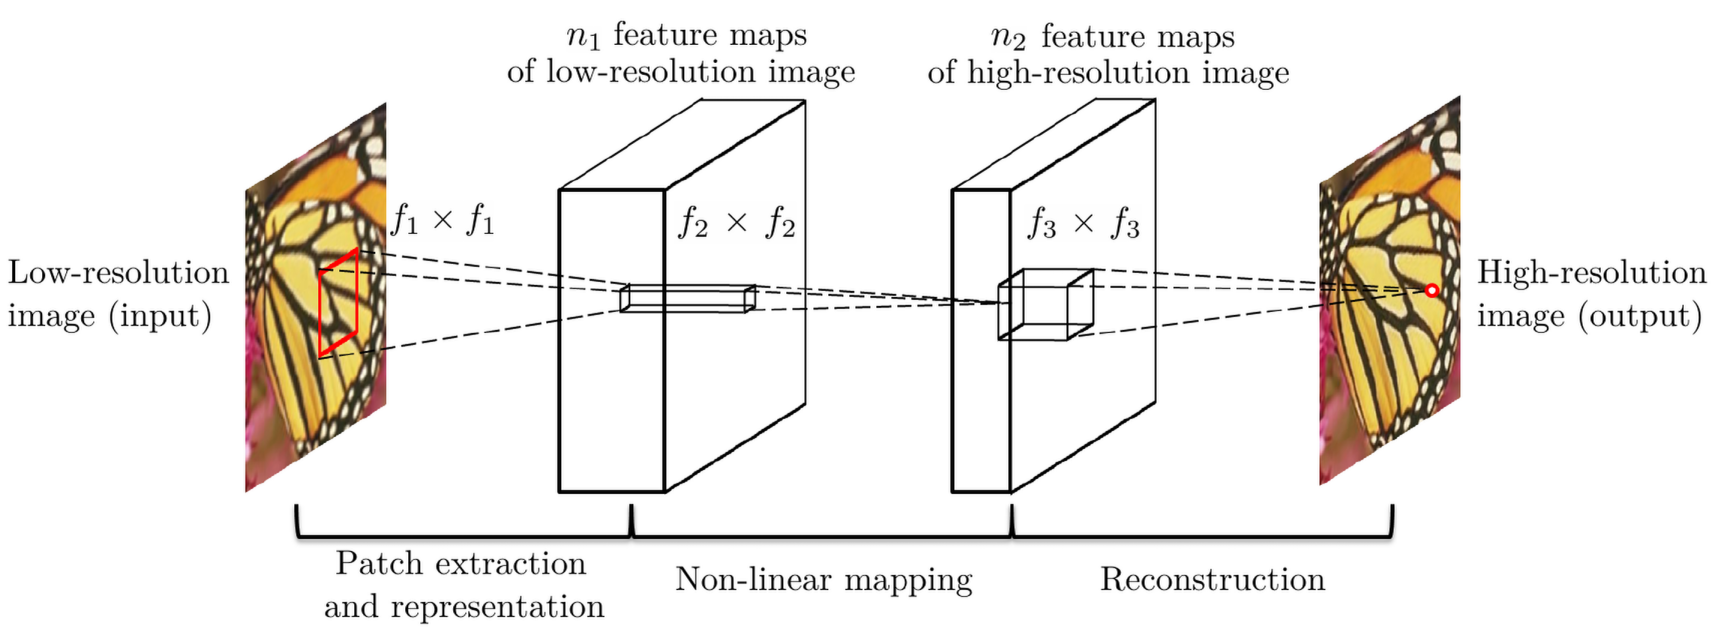
\includegraphics[width=0.8\columnwidth]{figures/architettura_SRCNN.png}
    \caption{Architettura della rete CNN, primo layer è per la feature extraction;
    il secondo per non-linear mapping
    e il terzo cerca di abbinare le predizioni della rete all'immagine ad alta risoluzione}

    \vspace{0.5cm}

    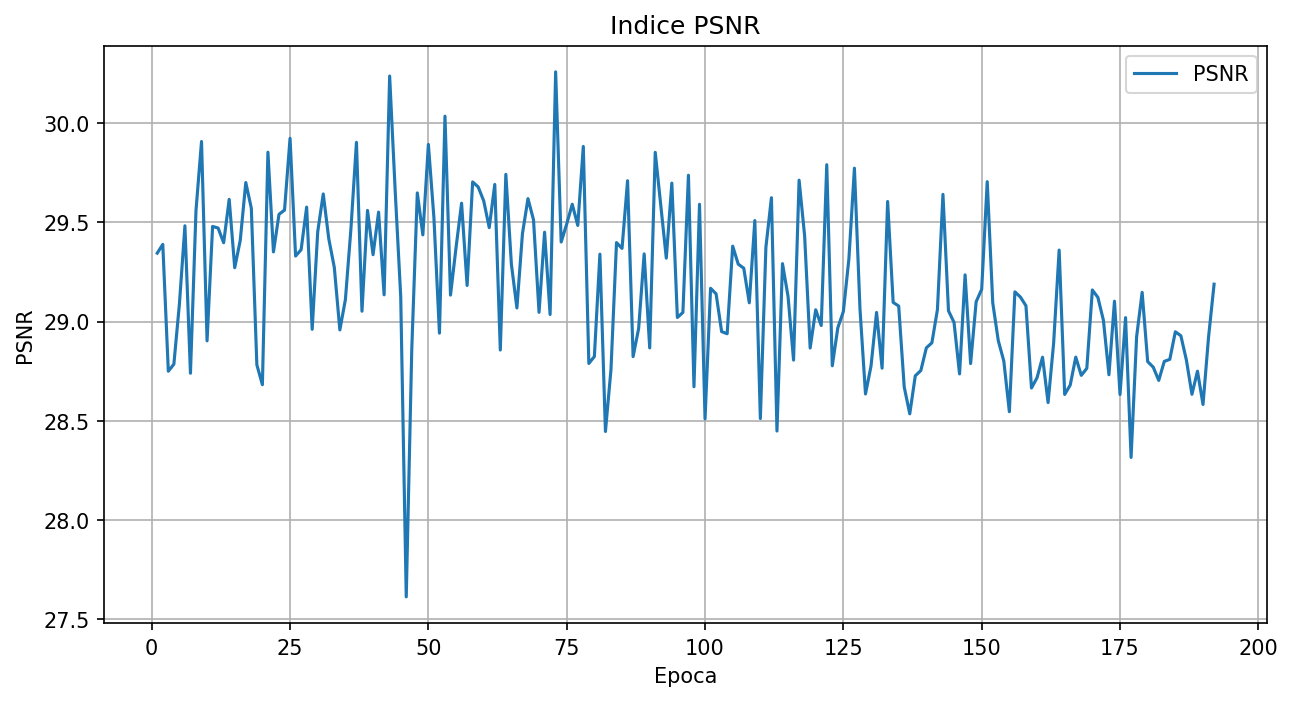
\includegraphics[width=0.8\columnwidth]{figures/srcnn_600_9-5-5-5-5-5-5_BN_L1_psnr_plot.png}
    \caption{Kernel: 5x5, BN, L1 Loss}

\end{figure}